% !TEX program = xelatex

\documentclass{beamer}
\usepackage[utf8]{inputenc}
\usepackage{listings}
\usepackage{fontspec} % 定制字体
\usepackage{xeCJK}
\usepackage{utopia} %font utopia imported
%\usepackage[UTF8,noindent]{ctexcap}
\usepackage{latexsym,amssymb,amsmath,amsbsy,amsopn,amstext,xcolor,multicol}
\usepackage{graphicx,wrapfig,fancybox}
\usepackage{booktabs}
% \usetheme{Rochester}
\usetheme{Madrid}
\usecolortheme{default}
\setmainfont{LinLibertine_R.otf}[
  BoldFont = LinLibertine_RZ.otf,
  ItalicFont = LinLibertine_RI.otf,
  BoldItalicFont = LinLibertine_RZI.otf]
\usepackage{xcolor} % 定制颜色
\definecolor{mygreen}{rgb}{0,0.6,0}
\definecolor{mygray}{rgb}{0.5,0.5,0.5}
\definecolor{mymauve}{rgb}{0.58,0,0.82}
\renewcommand{\thefootnote}{\fnsymbol{footnote}} %*, **, ***

%This block of code defines the information to appear in the
%Title page
\title[复试汇报] %optional
{清华大学计算机系研招 \\
复试汇报}

\author[芦迪] % (optional)
{芦迪}

\date[2019.3.16] % (optional)
{\today}

% \logo{
\includegraphics[height=1.5cm]{images/thuee-logo.png}}

%End of title page configuration block
%------------------------------------------------------------

%------------------------------------------------------------
%The next block of commands puts the table of contents at the 
%beginning of each section and highlights the current section:

\AtBeginSection[]
{
  \begin{frame}
    \frametitle{目录}
    \tableofcontents[currentsection]
  \end{frame}
}
%------------------------------------------------------------


\begin{document}
%The next statement creates the title page.
\frame{\titlepage}


%---------------------------------------------------------
%This block of code is for the table of contents after
%the title page
% \begin{frame}
% \frametitle{目录}
% \tableofcontents
% \end{frame}
%---------------------------------------------------------
\section{个人信息}
\begin{frame}{个人信息}
  \textbf{基本信息}:芦迪,男,22岁,河南信阳人

  \textbf{教育背景}:清华大学,电子工程系
  \begin{itemize}
    \item 就读时间:2014年8月--2018年7月
    \item 成绩排名:13/32,GPA:83/100
    \item 奖励情况:国家励志奖学金、社会工作优秀奖
    \item 所获学位:电子信息科学与技术,工学学士
  \end{itemize}
  \textbf{政治面貌}:共产党员
  \begin{itemize}
    \item 2017年6月加入中国共产党
  \end{itemize}
  \textbf{外语水平}:通过英语六级和清华英语水平一考试
\end{frame}

\section{项目经历}

\subsection{课程项目}
\begin{frame}{课程项目}
\textbf{安卓应用开发}
\begin{itemize}
  \item 读书笔记分享 App
  \item 主要负责内容:
  \begin{itemize}
    \item 软件需求分析
    \item 服务器与数据库的搭建
    \item 应用与服务器网络通信的实现
  \end{itemize}
  \item 被组内同学推选为小组MVP
\end{itemize}

\textbf{人脸表情识别项目}
\begin{itemize}
  \item 采用深度学习方法,使用 Caffe 框架
  \item 对公开数据集中人脸表情识别准确率达到了87.77\%
  \item 将人脸表情识别模型应用到视频情感分析中,取得了较好的结果
\end{itemize}
\end{frame}

\subsection{毕业设计}
\begin{frame}{毕业设计}
  \textbf{毕设题目}:基于解析数据的DNS安全评估与增强

  \textbf{主要工作}:
  \begin{itemize}
    \item 文献调研,了解研究现状,确认研究计划
    \item 数据获取:使用ZMap快速进行DNS查询,获取1000个域名在1.6万个开放解析器上的近千万条查询结果
    \item 数据处理:结合IP地址的AS号,使用聚类算法,对解析结果进行分类,离群点可认为是被干扰的结果
  \end{itemize}

  \begin{table}
    \tiny
    \begin{tabular}{r l l l}
      \toprule
      Country &IP & Counts & Domain Example\\
      \midrule
           
      IRAN &	10.10.34.34&131&bilibili.com\\
      UAE &	10.10.34.35&32&sex.com\\
      FINLAND &	0.0.0.0 & 27 &exosrv.com\\
      PORTUGAL &	0.0.0.0&19&badoo.com\\
      ROMANIA &	0.0.0.0&11&cnzz.com\\
      LATVIA &	0.0.0.0&11&duba.com\\
      SERBIA &	79.101.14.184&7&www.goal.com\\
      B\&H &	127.42.0.0& 7&hatenablog.com\\
      CYPRUS &	127.42.0.0&6&iqoption.com\\
      DENMARK &	80.239.178.184&5&hm.com\\
      \bottomrule
      \end{tabular}
      \caption{解析正确性判断结果示例}
  \end{table}
\end{frame}

\subsection{实习经历}

\begin{frame}{实习经历}
  \textbf{文通科技}:卷积神经网络的工程化
  \begin{itemize}
    \item 参考 Caffe 源码,实现了一个 CNN 的 Forward Model
    \begin{itemize}
      \item 包含卷积层、全连接层、池化层等
    \end{itemize}
    \item 实现了离线手写汉字识别的流程
    \item 实现了对Caffemodel的参数转化
    \item 无外部依赖,便于部署
  \end{itemize}
  \begin{figure}
    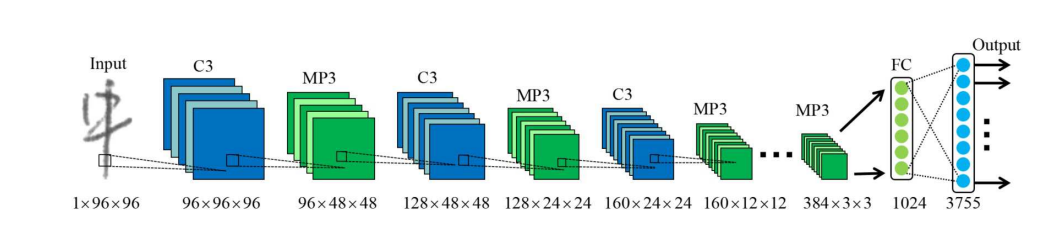
\includegraphics[height=2cm,width=9cm]{images/hccr_net.png}
    \caption{HCCR CNN 结构}
  \end{figure} 
\end{frame}


\begin{frame}{实习经历}
  \textbf{商汤科技}:人脸数据集管理与清洗
  \begin{itemize}
    \item 包含6000多万张人脸图片的数据集的管理与清洗
    \item 建立了一个对其进行高效保存、检索和使用的流程
    \begin{itemize}
      \item 实现了 attr2img、img2img等接口
    \end{itemize}
    \item 发布了一个按类别保存的人脸图片数据集,可用于分类训练
    \item 在按类别保存的人脸图片数据集上进行了进一步的去重、聚类
    \item 后期将使用此数据库对人脸解锁模型进行优化训练
  \end{itemize}
  \begin{figure}
    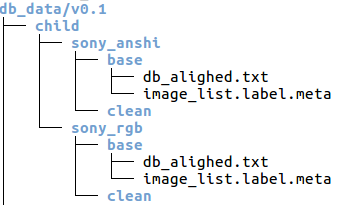
\includegraphics[height=3cm,width=5cm]{images/db_data_w.png}
    \caption{分类数据集示例}
  \end{figure} 
\end{frame}





\section{研究计划}

\begin{frame}{研究计划}
  \begin{itemize}
    \item 做过一些和计算机视觉相关的工作
    \item 当前深度学习技术在落地上存在一些问题:
    \begin{itemize}
      \item 对算力和功耗有要求,低功耗设备上难以部署
      \item 数据需求量大,难以在数据量少的领域应用
    \end{itemize}
    \item 希望能在推动新技术落地方面贡献力量
    \item 提高科研与工程能力,争取创造有价值的成果
  \end{itemize}
\end{frame}


\begin{frame}
  \begin{figure}
    
\includegraphics[height=4.46cm,width=8.58cm]{images/thank.jpg}
  \end{figure} 
\end{frame}
\end{document}

